\begin{figure}
    % First row
    \centering
    \begin{subfigure}{0.46\textwidth}
        \centering
        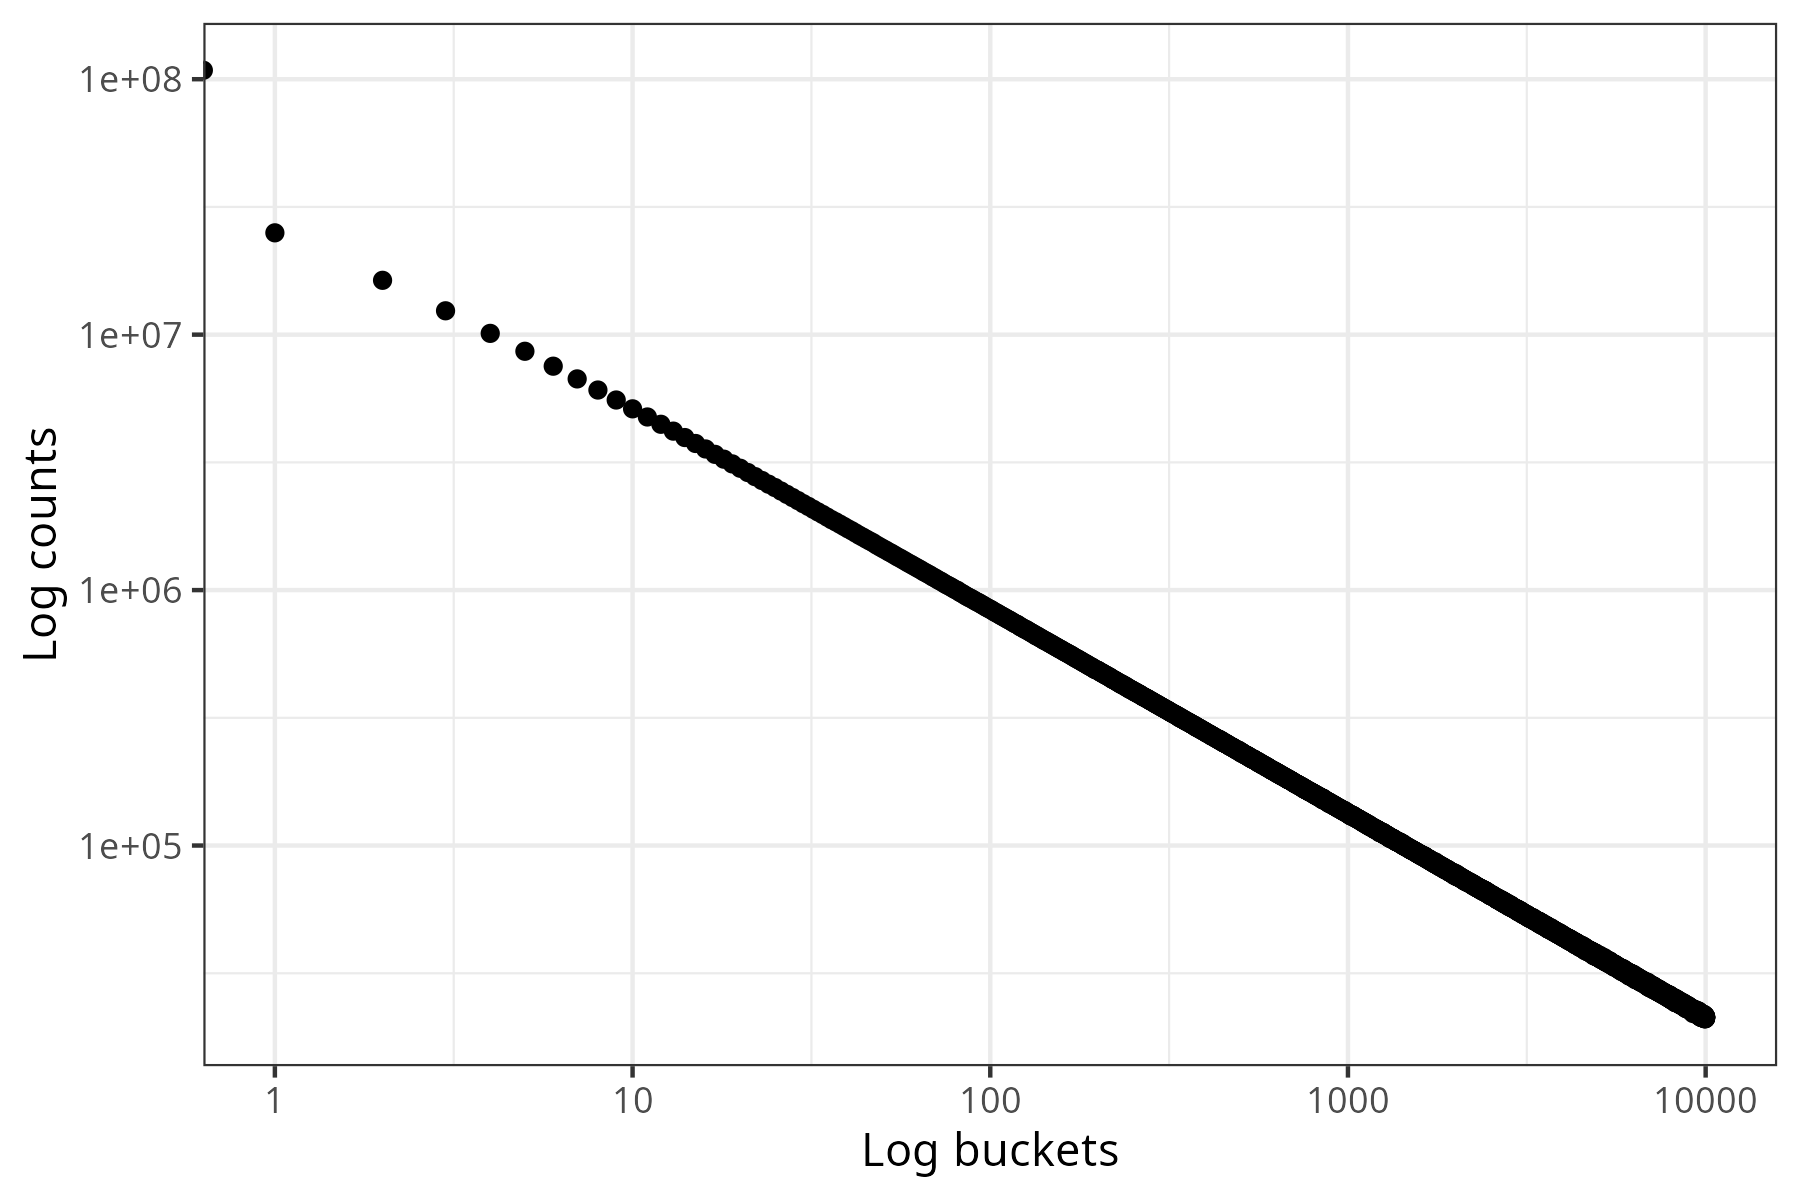
\includegraphics[width=\textwidth]{figures/log-log/apache.png}
        \caption{Rejection-Inversion}
    \end{subfigure}
    \hfill
    \begin{subfigure}{0.46\textwidth}
        \centering
        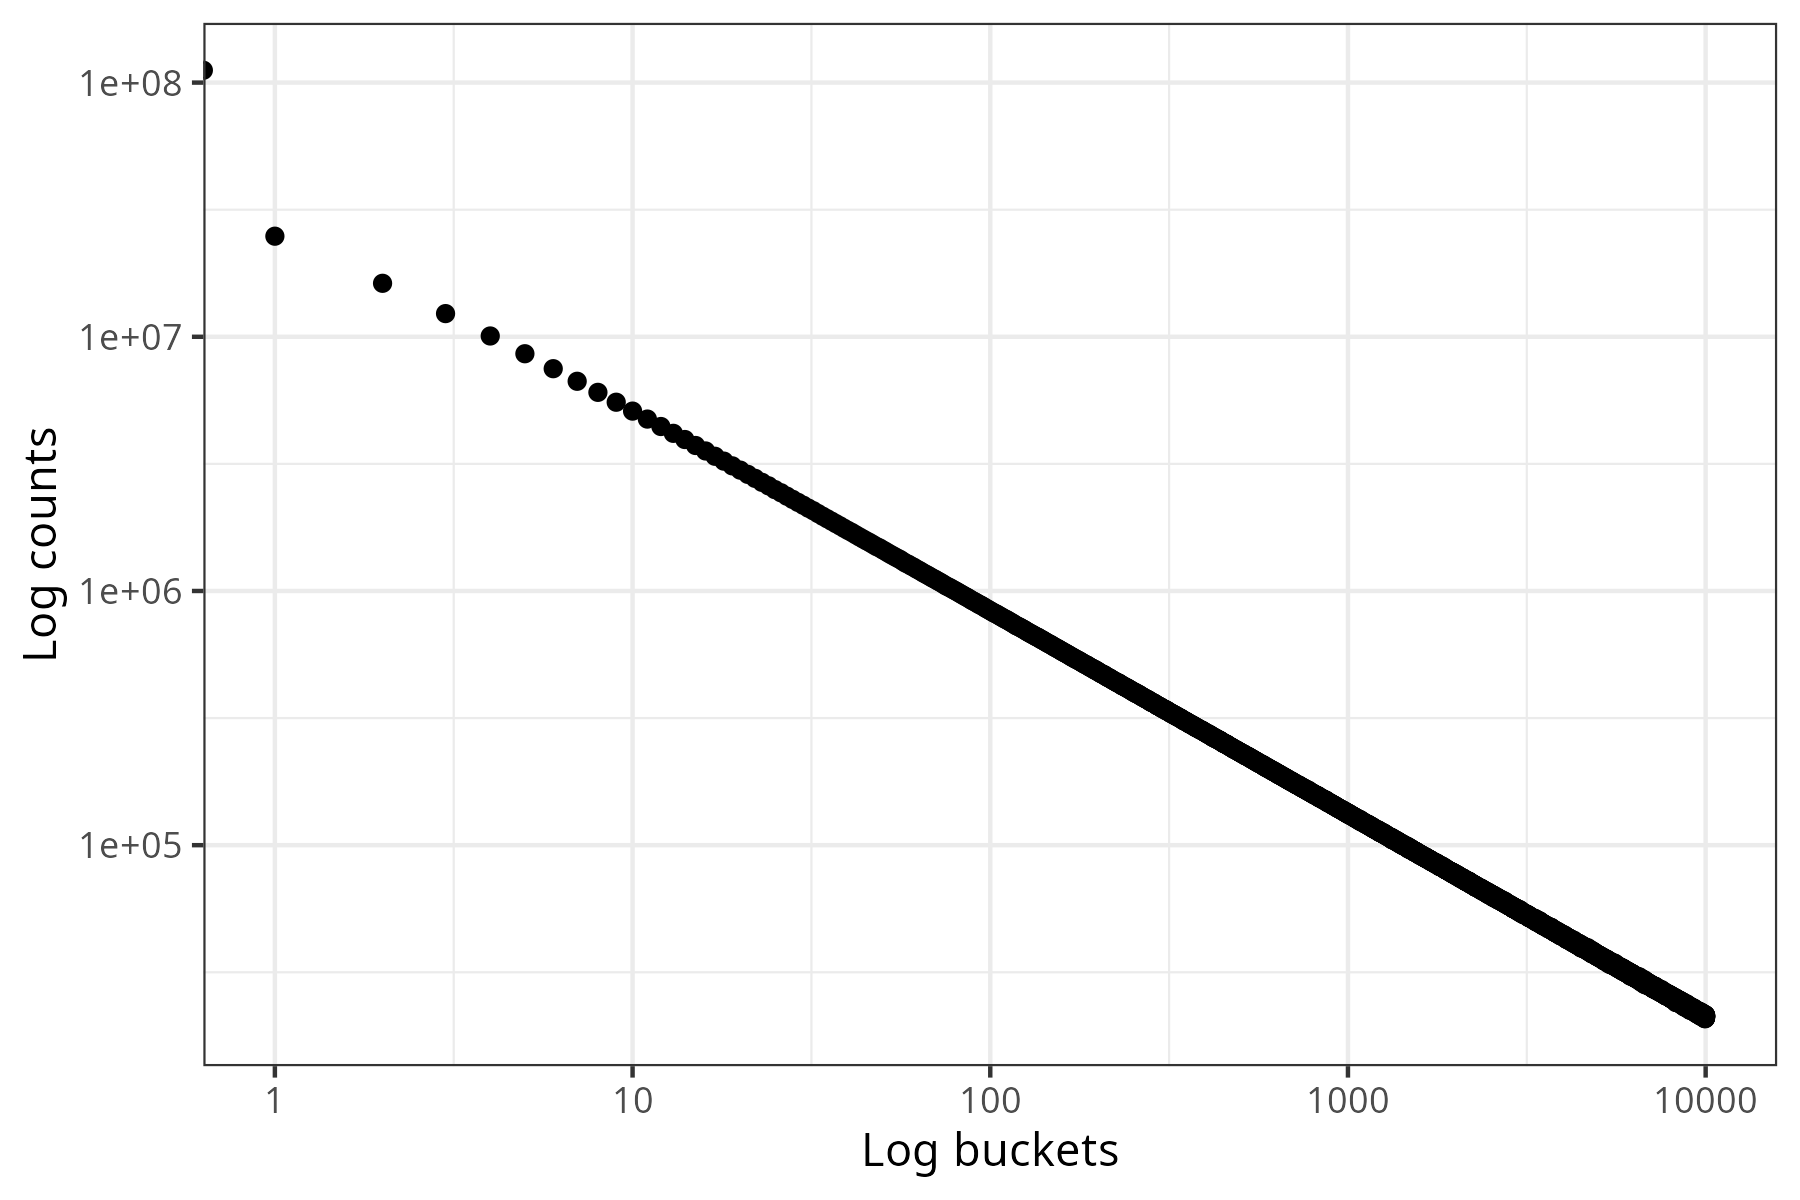
\includegraphics[width=\textwidth]{figures/log-log/ycsb.png}
        \caption{YCSB}
    \end{subfigure}
    
    \vspace{1em}

    % Second row
    \begin{subfigure}{0.46\textwidth}
        \centering
        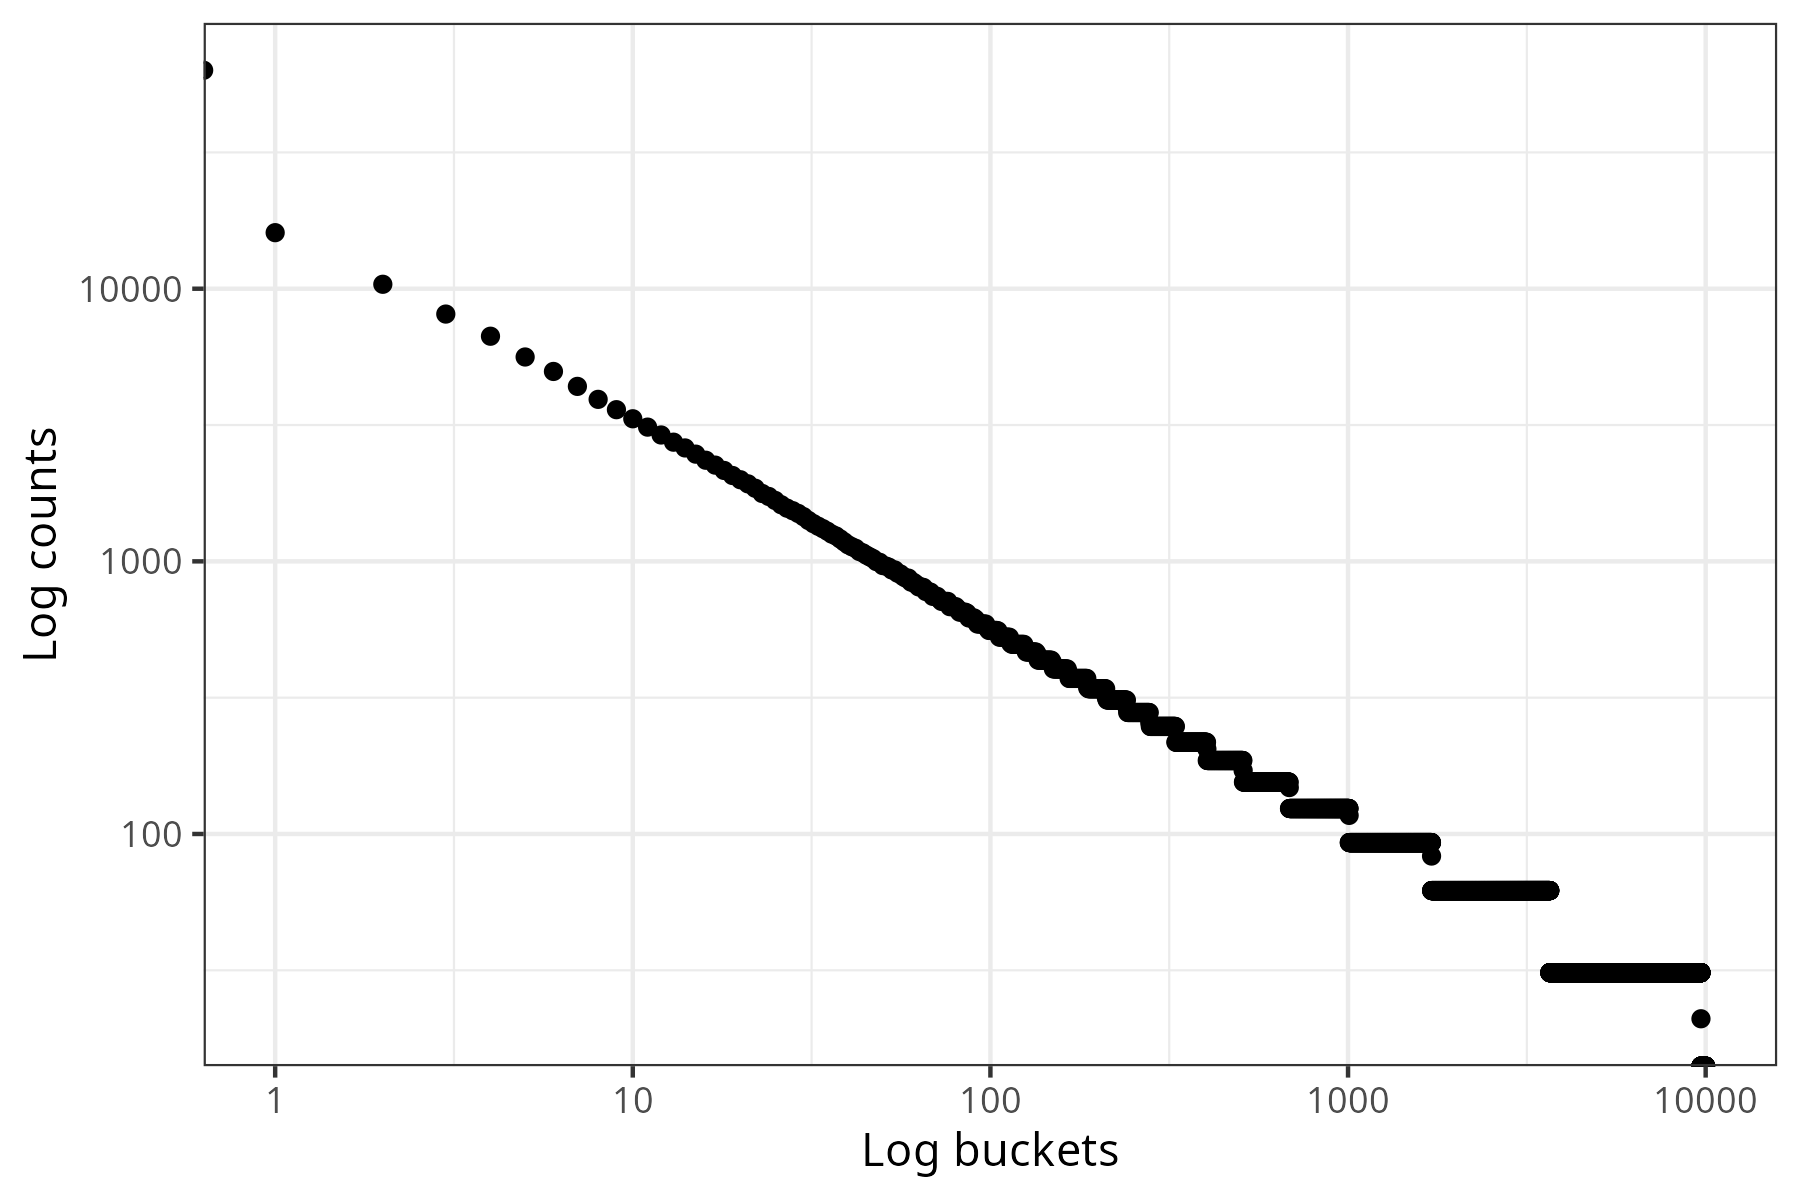
\includegraphics[width=\textwidth]{figures/log-log/fio.png}
        \caption{FIO}
    \end{subfigure}
    \hfill
    \begin{subfigure}{0.46\textwidth}
        \centering
        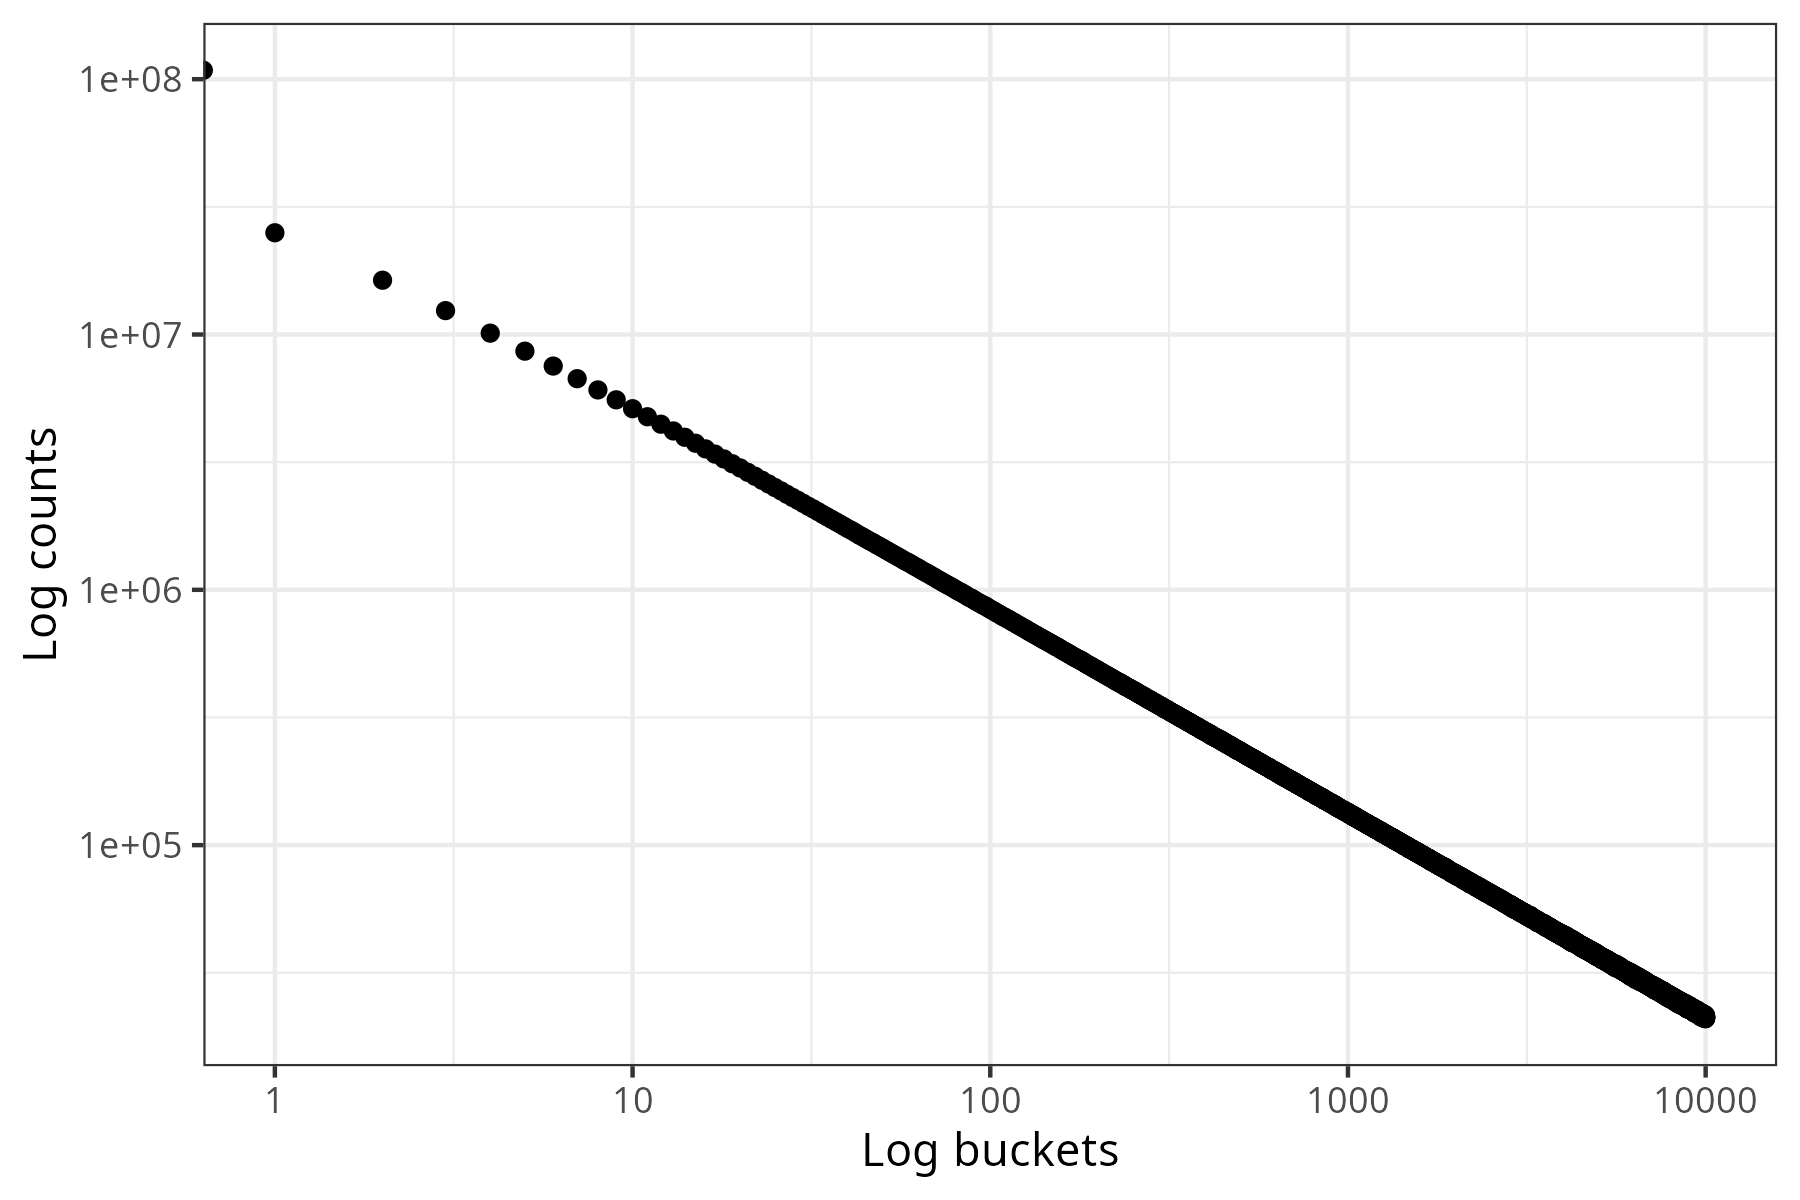
\includegraphics[width=\textwidth]{figures/log-log/sysbench.png}
        \caption{Sysbench}
    \end{subfigure}
    
    \vspace{1em}

    % Third row
    \begin{subfigure}{0.46\textwidth}
        \centering
        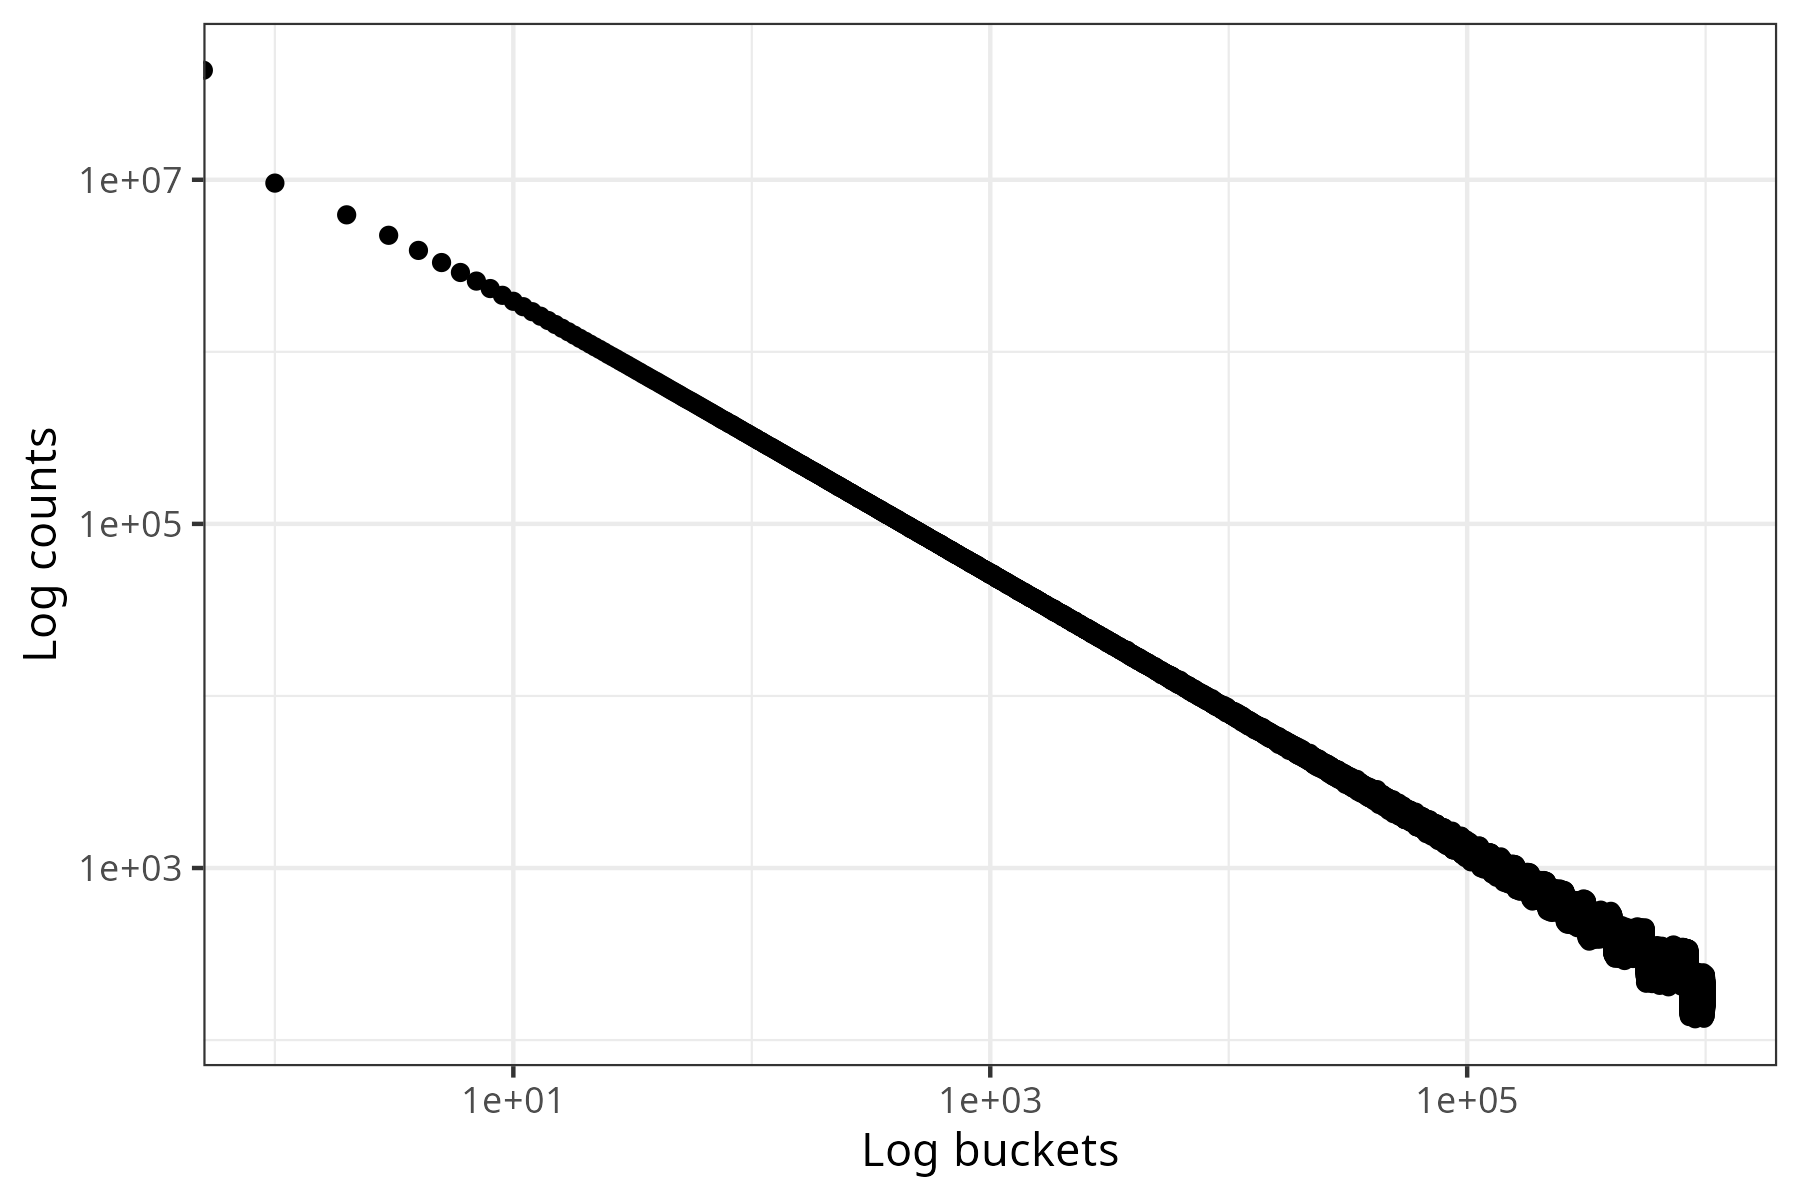
\includegraphics[width=\textwidth]{figures/log-log/marsaglia.png}
        \caption{Condensed Table Lookup}
    \end{subfigure}
    \hfill
    \begin{subfigure}{0.46\textwidth}
        \centering
        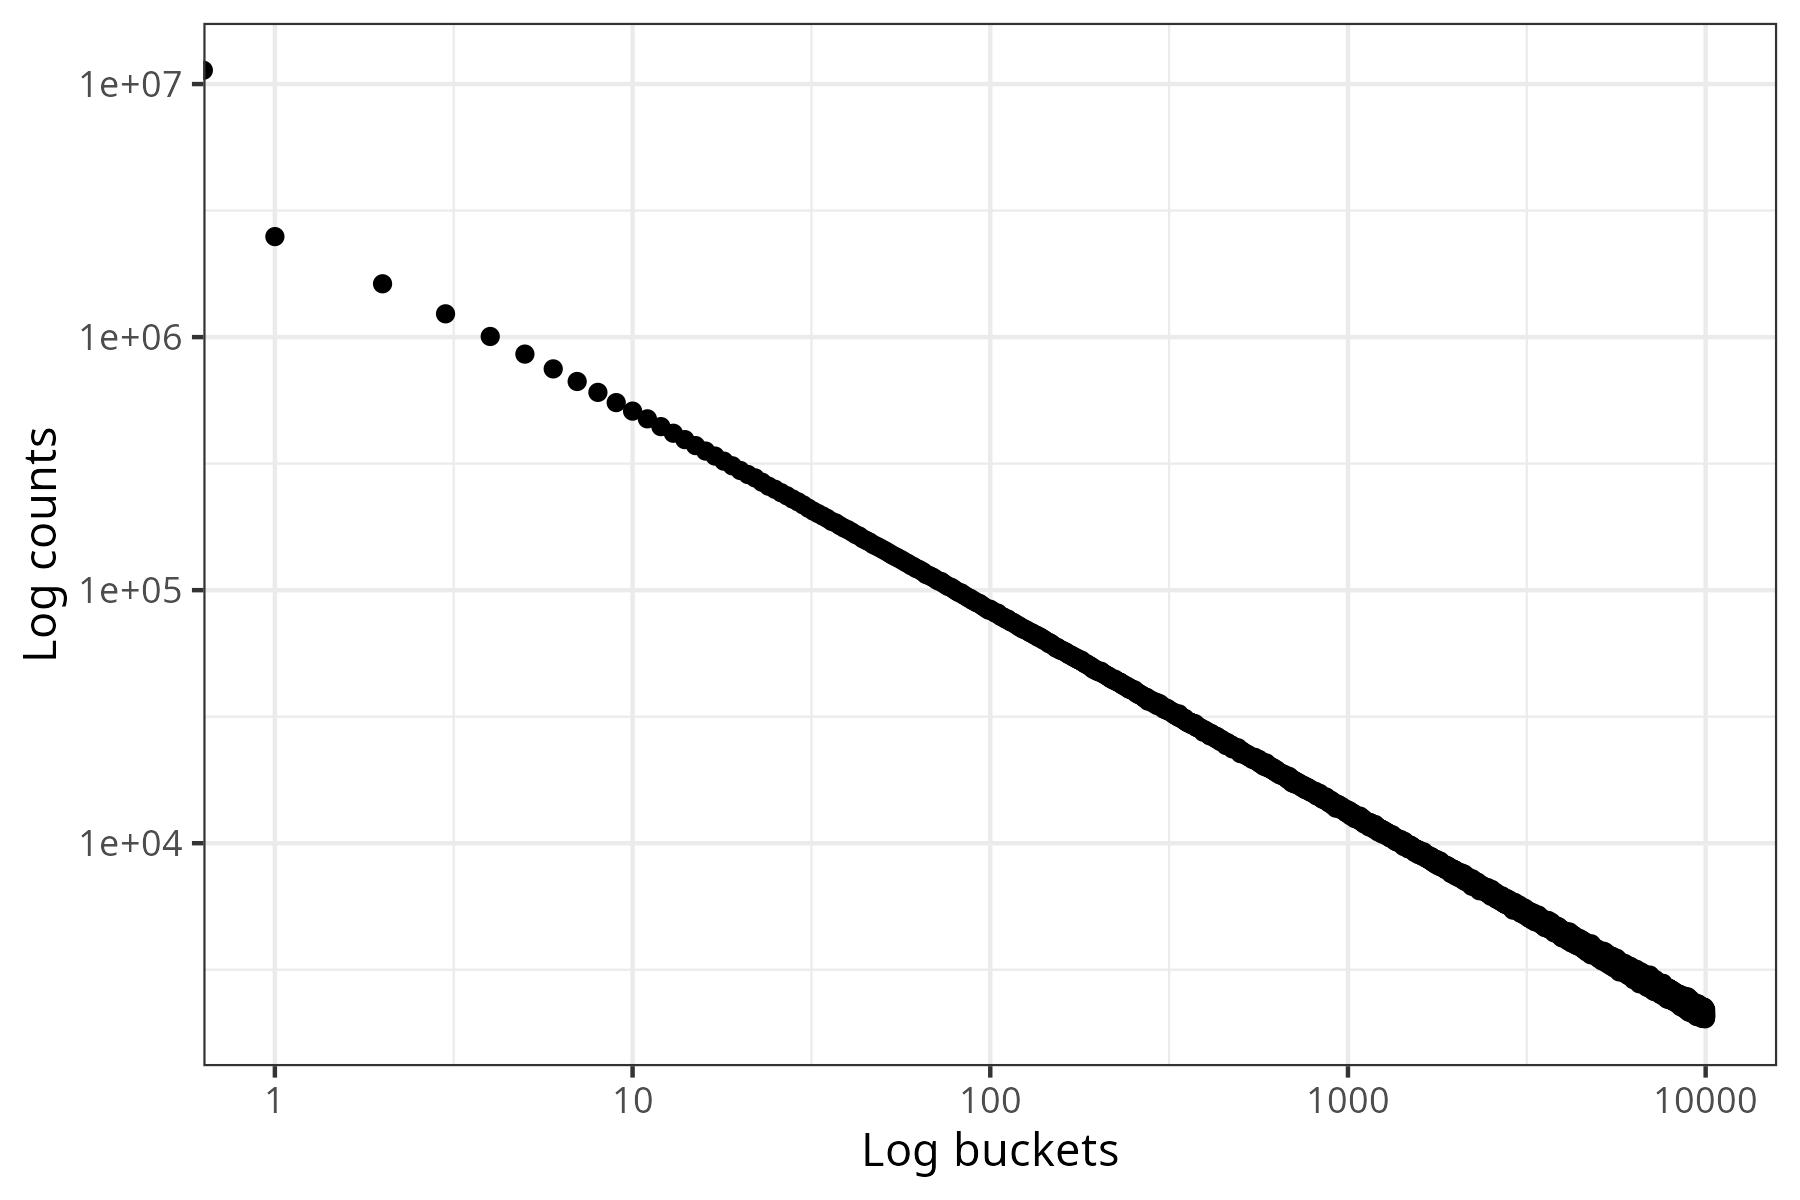
\includegraphics[width=\textwidth]{figures/log-log/rejection.png}
        \caption{Rejection Sampling}
    \end{subfigure}
    
    
    \caption{Log-log plots of the performance of the 6 different variate generators.}
    \label{fig:log-log}
\end{figure}